% !TeX encoding=utf8
% !TeX spellcheck = de_CH_frami

\chapter{BPM auf dem "`Raspberry PI"' in der Domäne "`Home Automation"'}
In diesem Kapitel wird analysiert wie Business Prozesse auf einem Raspberry PI implementiert, beziehungsweise automatisiert werden können. Dabei werden verschiedene Lösungskategorien aufgezeigt und erläutert.


\section{Der Raspberry PI}
\todo{Fix Footenotemarks}
\begin{figure}
  \centering
  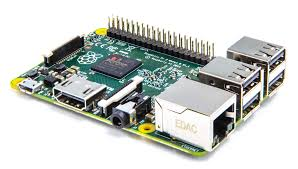
\includegraphics[width=6cm]{./images/RaspberryPi2ModelB}
  \captionsource{Raspberry Pi 2 Model B}{\url{https://www.raspberrypi.org/wp-content/uploads/2015/01/Pi2ModB1GB_-comp.jpeg}}
\end{figure}
  
Der Raspberry Pi ist ein Einplatinencomputer, welcher von der Raspberry Pi Foundation entwickelt und vertrieben wird. Er hat ungefähr die Grösse einer Kreditkarte und bietet zahlreiche On-Board Schnittstellen wie USB-, HDMI und Audio Anschlüsse (Abhängig vom konkreten Modell). Zusätzlich stehen eine bestimmte Anzahl an GPIO-Pins (General Purpose Input / Output) zur Verfügung. Mit Hilfe dieser Pins lassen sich zum einen Erweiterungs-Boards anschliessen und zum anderen können auch über ein spezielles Erweiterungsboard eigene Schaltungen, etc. gebaut und verlötet werden. Die Anzahl und genaue Funktion der einzelnen GPIO-Pins ist vom konkreten Raspberry PI Modell abhängig.

\begin{figure}[H]
  \centering
  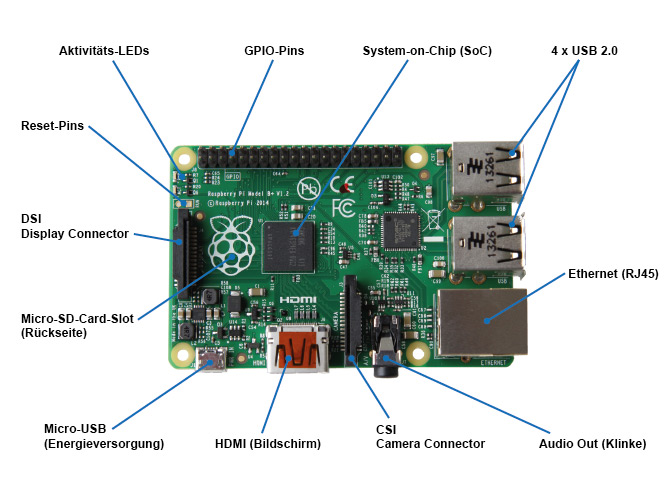
\includegraphics[width=13cm]{./images/RaspberryPi2ModelBPlusOverview}
  \captionsource{Raspberry Pi 2 Model B Überblick}{\url{https://www.elektronik-kompendium.de/sites/raspberry-pi/bilder/19052512.jpg}}
\end{figure}

\newpage
\begin{landscape}

\subsection{Raspberry Pi Modelle im Überblick}
\begin{table}[H]
\centering
\begin{tabular}{r | c  | c | c | c | c | c | c | c | c | c}
	& \THrot{\textbf{Raspberry Pi Model A}}
	& \THrot{\textbf{Raspberry Pi Model A+}}
	& \THrot{\textbf{Raspberry Pi Model B}}
	& \THrot{\textbf{Raspberry Pi Model B+}}
	& \THrot{\textbf{Raspberry Pi 2 Model B}}
	& \THrot{\textbf{Raspberry Pi 3 Model B}}
	& \THrot{\textbf{Raspberry Pi Compute}}
	& \THrot{\textbf{Raspberry Pi Zero}}\\
\midrule
Gewicht in Gramm
	& 	31
	&	23
	&	40		
	& 	45 
	&	40
	&	40
	&	7
	&	9\\
\midrule
System-on-a-Chip (SoC):
	& 	\multicolumn{4}{|c|}{BCM2835} 
	&	BCM2836
	&	BCM2837
	&	\multicolumn{2}{|c|}{BCM2835} \\
\midrule
CPU Kerne
	& 	1
	&	1
	&	1		
	& 	1 
	&	1
	&	4
	&	1
	&	1\\
\midrule
CPU Takt in MHz
	& 	\multicolumn{4}{|c|}{700} 
	&	900
	&	1200
	&	700
	&	1000\\
\midrule
CPU Architektur
	& 	\multicolumn{4}{|c|}{ARMv6 (32-bit)}  
	&	ARMv7 (32-bit)	
	&	ARMv7 (64-bit)	
	&	\multicolumn{2}{|c|}{ARMv6 (32-bit)}  	\\
\midrule
GPU Takt in MHz
	& 	\multicolumn{5}{|c|}{250} 
	&	300/400
	&	\multicolumn{2}{|c|}{250} \\
\midrule
Arbeitsspeicher in MB
	& 	\multicolumn{2}{|c|}{256}  
	&	256 / 512		
	& 	\multicolumn{2}{|c|}{512}  	
	& 	1024 
	&	\multicolumn{2}{|c|}{512}  	\\
	
\midrule
Pins
	& 	26
	&	40
	& 	26
	& 	\multicolumn{3}{|c|}{40}  	
	&	60
	&	40  	\\
	
\midrule
GPIO-Pins
	& 	17	
	&	26
	& 	17
	& 	\multicolumn{3}{|c|}{26}  	
	&	48
	&	26  	\\
\bottomrule
\end{tabular}
\end{table}

%Evtl.: http://praxistipps.chip.de/welcher-raspberry-pi-alle-modelle-im-vergleich_41923

\end{landscape}
\newpage

\section{Betrachteter Lösungsraum}
Ursprünglich wären folgende Einschränkungen für den Lösungsraum vorgesehen gewesen:
\blockquote {Da der Raspberry Pi eine offene Plattform ist, gibt es unterschiedlichste Möglichkeiten um das betrachtete Problem zu lösen. Im Kontext dieser Seminararbeit erfolgt die Betrachtung spezifisch für ein Raspberry Pi 2 Model B mit einem Raspbian OS (Debian Distribution für den Raspberry Pi). Als zusätzliche Prämisse gilt ebenfalls, dass der Kern der Anwendung auf dem Raspberry Pi lauffähig sein muss und die Lösung muss es in irgendeiner Form ermöglichen einen Ablauf / Prozess im Bereich Home Automation mit \gls{acr:BPMN} oder \gls{acr:BPEL} abzubilden. Alternative Lösungen, bei denen der Raspberry Pi als "`Client"' / "`Agent"' verwendet wird sind nicht im Fokus dieser Arbeit.}

Die ersten intensiven Recherchen haben gezeigt, dass es keine bis sehr wenige Lösungen gibt, welche den Grossteil der Anforderungen aus dem Lösungsraum erfüllen würden. Daher habe ich mich entschieden, den Lösungsraum anzupassen und zwei verschiedene Kategorien von Lösungen zu ermöglichen.

\textbf{Spezifische Home Automation Lösungen}
\begin{itemize}
\item Lauffähig auf dem Raspberry Pi mit Raspbian (32-Bit).
\item Fokus: Home-Automation
\item Funktionalität um Abläufe oder Aktionen zu automatisieren.
\item Eine Komponente
\item Open Source / Frei verfügbar (allenfalls Demoversion)
\item Muss via Web steuerbar sein.
\end{itemize}

\textbf{Lösung mit \gls{acr:BPMN}-Support im Bereich \gls{acr:IOT}}
\begin{itemize}
\item Lauffähig auf dem Raspberry Pi mit Raspbian (32-Bit).
\item Abläufe / Prozesse können mit Hilfe von \gls{acr:BPMN} modelliert werden.
\item Kann aus mehreren Komponenten bestehen
\item Möglichkeit zur Anbindung von \gls{acr:IOT}-Geräten aus dem Bereich "`Home Automation"' (z.B. via Plugins).
\item Open Source / Frei verfügbar (allenfalls Demoversion)
\end{itemize}


\section{Lösungen, Produkte \& Frameworks }
In diesem Abschnitt werden die recherchierten Lösungen, Produkte und Frameworks aufgezeigt. Diese Auflistungen sind nicht abschliessend und repräsentieren den Stand der Dinge zum Zeitpunkt der Recherchen im Q2/2016.

\subsection{Lösungskategorie: Spezifische Home Automation Lösungen}
Die Inhalte dieser Lösungskategorie wurden zum Grössten Teil aus dem Kapitel \ref{sec:Analyse:HA:LPF} \nameref{sec:Analyse:HA:LPF} entnommen und nach der Lauffähigkeit auf dem Raspberry Pi und Raspbian gefiltert.

\begin{itemize}
\item TriggerHappy
\item HomeAssistant
\item openHAB (2)
\item CastleOS
\item HomeGenie
\item Freedomotic
\item Domoticz
\end{itemize}

Filter-Kriterien: OpenSource, Kein Framework, mindestens Trigger \& Action Support, unter linux betreibbar
\begin{itemize}
\item TriggerHappy (Für Web-Services)
\item HomeAssistant (https://home-assistant.io/getting-started/)
\item openHAB (2)
\item CastleOS (Windows basiert)
\item HomeGenie
\item Freedomotic (http://www.freedomotic.com/content/download)
\item Domoticz
\end{itemize}

- OpenHAB: https://github.com/openhab/openhab/wiki/Z-Wave-Binding
- Evtl. mit ubidots (via HTTP-Request http://ubidots.com/docs/\#contents)
- HomeGenie: http://www.homegenie.it/
- Domoticz

\subsection{Lösung mit BPMN-Support im Bereich IOT}
Der definierte Lösungsraum dieser Lösungskategorie ermöglicht ein breites Spektrum an Lösungen. Nachfolgend werden einige der möglichen Lösungen aufgezeigt.

\begin{itemize}
\itemBfText{Activiti BPM (Java)}{}
\itemBfText{jBPM (Java)}{}
\itemBfText{Camunda (Java)}{https://github.com/zambrovski/mqtt-camunda-bpm} Nicht oben-Source
\itemBfText{Drools (java)} {}http://www.drools.org/ with jbpm
\itemBfText{http://www.bonitasoft.com/}{} Linux 64-Bit only
\itemBfText{http://www.imixs.org/}{}

\end{itemize}

https://bpmn.io/

% https://en.wikipedia.org/wiki/List_of_BPMN_2.0_engines

\begin{itemize}
\item Spezifische Lösung für den Raspberry PI -aus dem Bereiche BPM
\item Benutzung einer Lösung und Erweiterung
\item Kombination von Komponenten
% https://azure.microsoft.com/en-us/blog/build-an-azure-app-service-to-record-raspberry-pi-sensor-data/
% http://tonynysraspberrypi.blogspot.ch/
\item Komponente in übergreifenden Lösung
% https://www.eclipsecon.org/na2015/session/bpm-things-iot-and-processes
% http://column2.com/2015/03/bpmnext-2015-day-1-demos-sap-w4-and-whitestein/
% http://en.w4software.com/
\end{itemize}


\section{Realisierung eines Beispielhaften Prozesses mit BPMN im Bereich "`Home Automation"'}
Als Beispiel für diese Seminararbeit wird folgender Setup realisiert:


